\chapter[Autostati dell'operatore di posizione]{Autostati dell'operatore di posizione, misure di posizione e funzione d'onda\footnote{S1.6,1.7}}
Abbiamo assunto che le osservabili finora considerate abbiano uno spettro discreto di autovalori. In meccanica quantistica, tuttavia, vi sono \textbf{osservabili con autovalori continui}.\\
Un caso particolarmente importante di osservabile con spettro continuo è rappresentato dalla \textbf{posizione}.
Consideriamo (per semplicità) una particella vincolata a muoversi in una dimensione e sia $x$ l'asse lungo il quale è possibile il moto. Possiamo allora pensare di indicare con il simbolo $\ket{x'}$ \textbf{lo stato in cui la particella si trova nella posizione x}.
Una misura di posizione per una particella che si trovi nello spazio $\ket{x'}$ fornisce (per definizione) con certezza il valore $x'$. In altri termini, lo stato $\ket{x'}$ deve essere un \textbf{autostato dell'operatore di posizione} corrispondente all'autovalore $x'$.
\begin{equation}
  x\ket{x'} = x'\ket{x'} .
\end{equation}
In questa equazione $x'$ è semplicemente un numero mentre $x$ rappresenta \textbf{l'operatore posizione}.
Così come uno stato qualsiasi può essere sviluppato in serie di autostati di una grandezza con spettro discreto, allo stesso modo \textbf{uno stato può essere sviluppato}, questa volta in integrale, \textbf{secondo un sistema completo di autostati di una grandezza con spettro continuo}. Nel caso degli autostati dell'operatore posizione, questo sviluppo ha la forma
\begin{equation}
  \label{eq:cap5_1}
  \ket{\alpha} = \int_{-\infty}^{\infty}\dd{x'}\ket{x'}\braket{x'}{\alpha} .
\end{equation}
Contrariamente al caso di variabili con spettro discreto, il modulo quadro $\abs{\braket{x'}{\alpha}}^2$ non può essere interpretato come probabilità che una particella nello stato $\ket{\alpha}$ venga a trovarsi nella posizione $x'$. Infatti, per una variabile continua, tale probabilità è nulla.\\
Il significato fisico dell'ampiezza $\braket{x'}{\alpha}$ può essere derivato nel modo seguente.
Utilizzando lo sviluppo (\ref{eq:cap5_1}) calcoliamo il valore medio della posizione nello stato $\ket{\alpha}$
\begin{align}
  \ev{x}{\alpha} = \int_{-\infty}^{\infty}\dd{x'}\mel{\alpha}{x}{x'}\braket{x'}{\alpha}=\int_{-\infty}^{\infty}\dd{x'}x'\abs{\braket{x'}{\alpha}}^2 .
\end{align}
Da questa espressione vediamo che la quantità
\begin{equation}
  \abs{\braket{x'}{\alpha}}^2\dd x'
\end{equation}
rappresenta la probabilità che la particella nello stato $\ket{\alpha}$ si trovi posizionata in un intervallo di larghezza $\dd{x'}$ attorno al punto $x'$.\\
Per un intervallo infinitesimo, \textbf{la probabilità che una particella nello stato }$\ket{\alpha}$ \textbf{si trovi compresa in un intervallo di larghezza }$\dd{x'}$ \textbf{nell'intorno del punto }$x'$ \textbf{è}:
\begin{equation}
  P\qty(x'-\frac{\dd{x'}}{2}, x'+\frac{\dd{x'}}{2}) = \abs{\braket{x'}{\alpha}}^2\dd{x'} .
\end{equation}
Dall'equazione (\ref{eq:cap5_1}) risulta che questa probabilità è correttamente normalizzata
La probabilità di registrare la particella in qualche punto compreso tra $-\infty$ e $+\infty$ è data da $\int_{-\infty}^{+\infty}\dd{x'}\abs{\braket{x'}{\alpha}}^2$.
Dall'equazione (\ref{eq:cap5_1}) risulta che questa probabilità è correttamente normalizzata all'unità se lo stato $\ket{\alpha}$ è normalizzato:
\begin{equation}
  \label{eq:cap5_2}
  \int_{-\infty}^{+\infty}\dd{x'}\abs{\braket{x'}{\alpha}}^2 = \int_{-\infty}^{+\infty}\dd{x'}\braket{\alpha}{x'}\braket{x'}{\alpha}=\braket{\alpha}{\alpha} = 1 .
\end{equation}
Solitamente il prodotto scalare $\braket{x'}{\alpha}$ prende la denominazione di \textbf{funzione d'onda} $\psi_{\alpha}\qty(x')$ per lo stato $\ket{\alpha}$
\begin{equation}
  \braket{x'}{\alpha} = \psi_{\alpha}\qty(x')
\end{equation}
L'equazione (\ref{eq:cap5_2}) esprime la \textbf{condizione di normalizzazione per la funzione d'onda}
\begin{equation}
  \int_{\infty}^{+\infty}\dd{x'}\abs{\psi_{\alpha}\qty(x')}^2=1 .
\end{equation}
Utilizzando l'equazione (\ref{eq:cap5_1}), che definisce la relazione di completezza degli autostati della posizione, \textbf{è possibile esprimere una qualunque ampiezza} $\braket{\beta}{\alpha}$ \textbf{in termini di un integrale di sovrapposizione delle funzioni d'onda per gli stati} $\ket{\beta}$ \textbf{ed} $\ket{\alpha}$:
\begin{equation}
  \int_{\infty}^{+\infty}\dd{x'}\braket{\beta}{x'}\braket{x'}{\alpha} = \int_{\infty}^{+\infty}\dd{x'} \psi^*_{\beta}\qty(x')\psi_{\alpha}\qty(x') .
\end{equation}
Similmente, lo sviluppo di un vettore di stato $\ket{\alpha}$ in autostati di un osservabile con spettro discreto $A$,
\begin{equation}
  \ket{\alpha} = \sum_{a'}\ket{a'}\braket{a'}{\alpha}\equiv \sum_{a'}C_{a'}\ket{a'} ,
\end{equation}
può essere espresso in termini di uno \textbf{sviluppo della funzione d'onda} $\psi_{\alpha}$ \textbf{in "autofunzioni" dell'operatore $A$}.
Moltiplicando la precedente equazione a sinistra per il bra $\bra{x'}$ si ottiene infatti:
\begin{equation}
  \psi_{\alpha}\qty(x') = \sum_{a'}C_{a'}u_{a'}\qty(x') ,
\end{equation}
dove si sono introdotte le \textbf{autofunzioni} dell'operatore $A$ corrispondenti agli autovalori $a'$:
\begin{equation}
  u_{a'}\qty(x') = \braket{x'}{a'} .
\end{equation}
\section[Normalizzazione degli autostati dell'operatore di posizione e funzione Delta di Dirac]{Normalizzazione degli autostati dell'operatore di posizione e funzione Delta di Dirac\footnote{ S1.6,1.7,LL5}}
Più complessa che nel caso dello spettro discreto è la questione della \textbf{normalizzazione degli autostati di osservabili con spettro continuo}
 ed in particolare, dunque, dell'operatore di posizione.
 Per dedurre la condizione di normalizzazione moltiplichiamo a sinistra l'equazione (\ref{eq:cap5_1}) per un autostato della posizione:
 \begin{equation}
   \label{eq:cap5_3}
   \braket{x'}{\alpha} = \int_{-\infty}^{+\infty}\dd{x''}\braket{x'}{x''}\braket{x''}{\alpha} .
 \end{equation}
Questa equazione deve valere per $\braket{x'}{\alpha}$ arbitrari e deve quindi essere un'identità. A tale scopo è necessario, anzitutto, che il coefficiente di $\braket{x''}{\alpha}$, cioè l'ampiezza $\braket{x'}{x''}$ si annulli per tutti gli $x'\neq x''$. Per $x'=x''$, questa ampiezza deve diventare infinita; viceversa l'integrale in $\dd{x''}$ semplicemente nullo. In tal modo, l'ampiezza $\braket{x'}{x''}$ è una funzione della differenza $x'-x''$, che si annulla allorché questa differenza è diversa da zero e diventa infinita allorché questa è nulla. Indichiamo questa funzione con $\delta\qty(x'-x'')$
\begin{equation}
  \braket{x'}{x''} = \delta\qty(x'-x'') .
\end{equation}
Il modo in cui la funzione $\delta\qty(x'-x'')$ diventa infinita per $x'-x''=0$ è determinato dall'equazione (\ref{eq:cap5_3}) che possiamo scrivere in forma generale come
\begin{equation}
  f\qty(x_0) = \int_{-\infty}^{+\infty}\dd{x}\delta\qty(x-x_0)f\qty(x) .
\end{equation}
È ovvio che a questo scopo si deve avere in particolare
\begin{equation}
  \int_{-\infty}^{+\infty}\dd{x}\delta\qty(x-x_0) = 1 .
\end{equation}
La funzione così definita si chiama \textbf{funzione $\delta$ di Dirac}.
Riepiloghiamo le formule che la definiscono
\begin{align}
  \delta(x) = 0 \quad \text{per }x\neq 0 ; \\
  \delta(0) = \infty ; \\
  \int_{-\infty}^{+\infty}\dd{x}\delta(x)=1 .
\end{align}
È ovvio che come limiti di integrazione nell'ultima equazione si possono prendere due altri valori qualsiasi tra cui è compreso il punto $x=0$.
Presentiamo qui alcune possibili definizioni della $\delta$ di Dirac come limite di funzioni ordinarie
\begin{itemize}
\item
\begin{tabular}{ >{\centering\arraybackslash} m{1.5cm} >{\centering\arraybackslash} m{3.5cm} >{\centering\arraybackslash} m{4.5cm}}
$\displaystyle{\lim _{a \rightarrow 0}}$ & 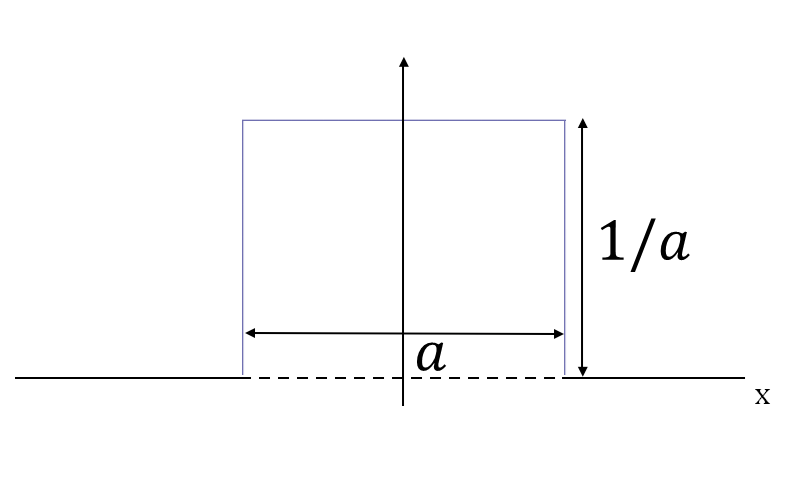
\includegraphics[width=3.5cm]{immagini/cap_5/fig_5_1.png}  & $=\displaystyle{\begin{cases}
1/a \textrm{ per } \vert x \vert \leq a/2\\
0 \textrm{ per } \vert x \vert > a/2
\end{cases}}$
\end{tabular}
\item
\begin{tabular}{ >{\centering\arraybackslash} m{4cm} >{\centering\arraybackslash} m{3.5cm} >{\centering\arraybackslash} m{2cm}}
$\displaystyle{\lim _{a \rightarrow 0}\frac{1}{a\sqrt{\pi}}e^{-x^2/a^2}=}$ & 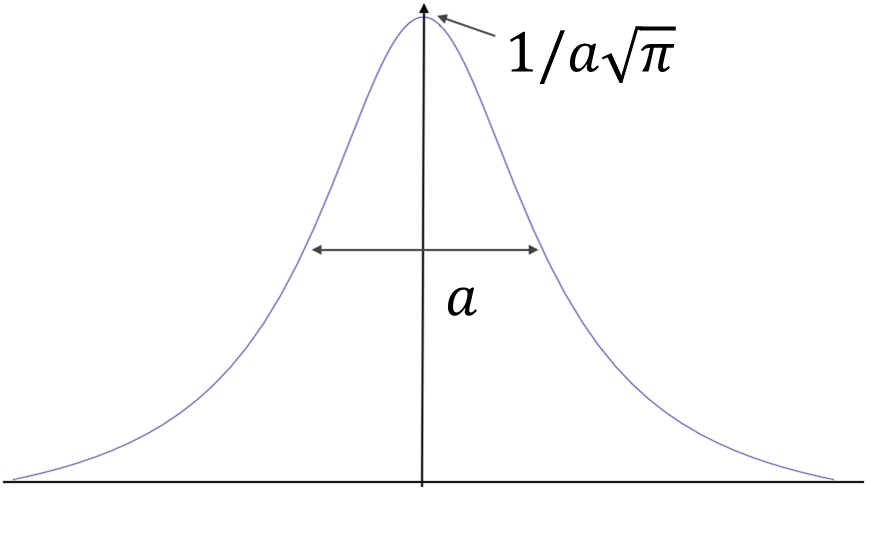
\includegraphics[width=3.5cm]{immagini/cap_5/fig_5_2.png}  & (gaussiana)
\end{tabular}
\item 
\begin{tabular}{ >{\centering\arraybackslash} m{4cm} >{\centering\arraybackslash} m{3.5cm} >{\centering\arraybackslash} m{2cm}}
$\displaystyle{\lim _{a \rightarrow 0}\frac{1}{\pi}\frac{a^2}{x^2+a^2}}=$ & 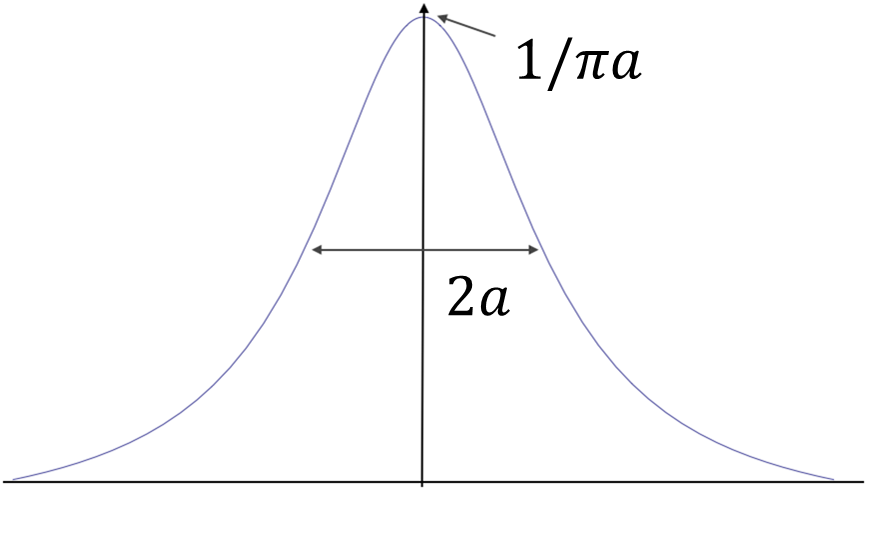
\includegraphics[width=3.5cm]{immagini/cap_5/fig_5_3.png}  & (lorentziana)
\end{tabular}
\item 
\begin{tabular}{ >{\centering\arraybackslash} m{4cm} >{\centering\arraybackslash} m{3.5cm} >{\centering\arraybackslash} m{2cm}}
$\displaystyle{\lim _{a \rightarrow 0}\frac{\sin(x/a)}{\pi x}}=$ & 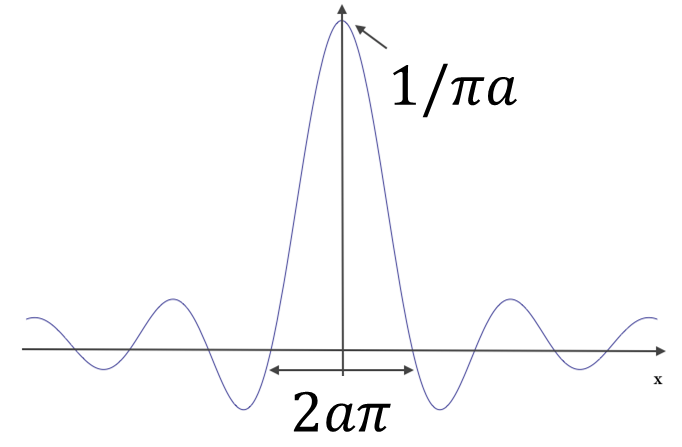
\includegraphics[width=3.5cm]{immagini/cap_5/fig_5_4.png}  & 
\end{tabular}
\end{itemize}
Dall'ultima definizione segue anche la rappresentazione integrale della $\delta$ di Dirac:
\begin{equation}
  \delta\qty(x) = \lim_{a\to0}\frac{\sin{x/a}}{\pi x}=\lim_{a\to0}\frac{1}{2\pi}\int_{-\frac{1}{a}}^{\frac{1}{a}}\dd{k}e^{ikx} ,
\end{equation}
ossia
\begin{equation}
  \delta(x)=\frac{1}{2\pi}\int_{-\infty}^{\infty}\dd{x}e^{ikx} .
\end{equation}
\section{Operatori nella rappresentazione delle coordinate}
In precedenza abbiamo discusso come una qualsiasi ampiezza $\braket{\beta}{\alpha}$ possa esprimersi in termini di un integrale di sovrapposizione delle funzione d'onda $\psi_{\beta}$ e $\psi_{\alpha}$ degli stati $\ket{\beta}$ e $\ket{\alpha}$.
Esaminiamo ora come gli \textbf{elementi di matrice} $\mel{\beta}{A}{\alpha}$ possano essere scritti usando le funzioni d'onda $\psi_{\beta}$ e $\psi_{\alpha}$. Si ha evidentemente:
\begin{align}
  \label{eq:cap5_4}
  \mel{\beta}{A}{\alpha} &= \int\dd{x'}\int\dd{x''}\braket{\beta}{x'}\mel{x'}{A}{x''}\braket{x''}{\alpha} =\nonumber\\
  &= \int\dd{x'}\int\dd{x''} \psi_{\beta}^*\qty(x')\mel{x'}{A}{x''}\psi_{\alpha}\qty(x'') .
\end{align}
L'ampiezza $\mel{\beta}{A}{\alpha}$ è dunque completamente determinata in termini di un integrale contenente le funzioni d'onda $\psi_{\beta}$ e $\psi_{\alpha}$ e gli elementi di matrice $\mel{x'}{A}{x''}$. Questi sono detti \textbf{elementi di matrice dell'operatore $A$ nella rappresentazione delle coordinate e sono, in generale, una funzione delle due variabili $x'$ e $x''$}.
Una notevole semplificazione si ha quando l'osservabile $A$ è una funzione dell'operatore posizione $X$. Consideriamo per esempio il caso in cui
\begin{equation}
  A= x^2 .
\end{equation}
Abbiamo allora:
\begin{equation}
  \mel{x'}{x^2}{x''} = \bra{x'}\qty(x''^2\ket{x''}) = x''^2\delta\qty(x'-x'') = x'^2\delta\qty(x'-x'') ,
\end{equation}
dove si è usato il fatto che $\ket{x''}$ è un autostato dell'operatore $x$ corrispondente all'autovalore $x''$ e la condizione di normalizzazione degli autostati di posizione. Sostituendo questo risultato nell'equazione (\ref{eq:cap5_4}) l'integrale doppio si riduce ad un integrale semplice in virtù delle proprietà della funzione $\delta$:
\begin{align}
  \mel{\beta}{x^2}{\alpha} &=\int\dd{x'}\int\dd{x''} \psi_{\beta}^*\qty(x')x'^2\delta\qty(x'-x'')\psi_{\alpha}\qty(x'') =\nonumber\\
  &= \int\psi_{\beta}^*\qty(x')x'^2\psi_{\alpha}\qty(x') .
\end{align}
In generale per un operatore funzione del solo operatore posizione $x$ si ha:
\begin{equation}
  \mel{\beta}{f(x)}{\alpha} = \int\dd{x'}\psi_{\beta}^*\qty(x')f\qty(x')\psi_{\alpha}\qty(x') .
\end{equation}
Si noti che $f(x)$ primo membro di queste equazioni è un operatore, mentre $f\qty(x')$ nel secondo membro non è un operatore.
\section[Regole di commutazione per gli operatori di posizione]{Regole di commutazione per gli operatori di posizione \footnote{S1.6}}
Le proprietà dell'operatore posizione sin qui considerate possono essere facilmente generalizzate al caso di tre dimensioni spaziali.
Possiamo indicare con il simbolo $\ket{\va{x}'}$ \textbf{il vettore di stato di una particella che si trovi nel punto di coordinate $\va{x}'= \qty(x',y',z')$}.
Una misura di posizione per una particella che si trovi nello stato $\ket{\va{x}'}$ fornisce con certezza i valori $x'$, $y'$ e $z'$ per le tre coordinate spaziali rispettivamente. In altri termini il vettore di stato $\ket{\va{x}'}$ è autostato simultaneo delle osservabili $x$, $y$ e $z$:
\begin{equation}
  x\ket{\va{x}'}=x'\ket{\va{x}'},\quad y\ket{\va{x}'}=y'\ket{\va{x}'},\quad z\ket{\va{x}'}=z'\ket{\va{x}'} .
\end{equation}
Sappiamo che per poter considerare un autostato simultaneo di $x$, $y$, e $z$ dobbiamo assumere che le tre componenti del vettore posizione possano essere misurate simultaneamente con un grado di precisione arbitrario. Dobbiamo perciò avere
\begin{equation}
  \comm{x_i}{x_j}= 0 ,
\end{equation}
dove $x_1$, $x_2$ ed $x_3$ stanno per $x$, $y$ e $z$ rispettivamente.